\documentclass[10pt,twocolumn]{article}

% use the oxycomps style file
\usepackage{oxycomps}
\usepackage{listings}
\usepackage{minted}
\usepackage{graphicx}
\graphicspath{ {./images/} }

% usage: \fixme[comments describing issue]{text to be fixed}
% define \fixme as not doing anything special
\newcommand{\fixme}[2][]{#2}
% overwrite it so it shows up as red
\renewcommand{\fixme}[2][]{\textcolor{red}{#2}}
% overwrite it again so related text shows as footnotes
%\renewcommand{\fixme}[2][]{\textcolor{red}{#2\footnote{#1}}}

% read references.bib for the bibtex data
\bibliography{Tiffany Mo}

% include metadata in the generated pdf file
\pdfinfo{
    /Title (Phishing Simulators for Cyber Awareness)
    /Author (Tiffany Mo)
}

% set the title and author information
\title{Gone Phishing: A Browser Game for Cyber-Awareness}
\author{Tiffany Mo}
\affiliation{Occidental College}
\email{tmo@oxy.edu}

\begin{document}

\maketitle

\section{Introduction} 
Phishing remains one of the most common forms of cybercrime and social engineering. Phishing attacks target users through deceptive messages that impersonate trusted institutions in order to steal sensitive information. While technical defenses like spam filters and firewalls are important, phishing continues to succeed because it most often exploits human behavior—urgency, authority, and familiarity—rather than technological vulnerabilities. As phishing tactics become more sophisticated, there is a growing need for interactive, engaging educational tools that teach users how to recognize and respond to social engineering threats. Traditional cybersecurity awareness efforts, such as training modules, email bulletins, and static videos, often struggle to hold users' attention and rarely offer hands-on practice.
This paper reviews prior research on the engineering of phishing, why they work, and their consequences. This review will also explore related educational games and their effectiveness. Building on this foundation, I plan to build a browser-based game, Gone Phishing, to help players identify phishing attacks. Unlike traditional cybersecurity training modules, Gone Phishing engages users through an active learning experience that simulates real-world decision-making. Players will take on the role of a fish navigating an ocean filled with phishing “bait,” each representing different phishing types such as whaling, spear phishing, and angler phishing. This game will also leverage AI, specifically OpenAI’s GPT-4o, to generate realistic phishing emails based on patterns extracted from real-world datasets like PhishTank. Emails will be tailored to resemble scenarios familiar to students, increasing their relevance and effectiveness. By integrating live AI generation, real phishing tactics, and engaging design, my project aims to make cybersecurity awareness both accessible and impactful for its players.
\section{{Problem Context}}

\subsection{What is Phishing?}
Phishing is a method used by cyber-criminals to trick users into disclosing sensitive information through seemingly legitimate emails. \cite{comprehensive_review} Attackers typically impersonate trusted entities—such as banks, employers, or government agencies—through emails, text messages, or fake websites. These messages often create a sense of urgency, pressuring victims to click malicious links, download harmful attachments, or enter credentials on fraudulent sites.

\subsection{Spear Phishing}
Spear phishing is a more specified and sophisticated type of phishing attack usually aimed at a specific group or individual.

\subsection{Smishing}
Smishing is a phishing attack that utilizes phone instead of written communication. This includes fraudulent SMS messages and calls. 

\subsection{Whaling}
Whaling is a subtype of spear phishing that exclusively targets high-profile executives to gain access to highly sensitive data from an organization. 

\subsection{Angler Phishing}
Angler phishing is similar to smishing, as it involves using social media to directly message targeted individuals on platforms like Facebook and Instagram. 

\subsection{Why is Phishing Important?}
The security of any organization relies on confidentiality, integrity, and availability. \cite{comprehensive_review} 
In order to maintain confidentiality, access to restricted and sensitive information must be restricted to authorized users. Phishing often targets login credentials for email, banking, or workplace accounts. Once attackers gain access to this information, they can steal personal data, send fraudulent messages, or escalate privileges within an organization, leading to identity theft or further breaches. If the identities of these authorized users are stolen, the attacker will be able to bypass the restrictions in place that prevent external adversaries from accessing sensitive information.
Access to such information allows for ransomware attacks, malware that encrypts the victim's data until the ransom is paid, that disrupt critical infrastructure and/or cause financial and reputational damage. Critical infrastructure refers to the fundamental facilities and systems that act as the backbone of a nation's economy, security, and health. There are 16 critical infrastructure sectors: chemical, commercial facilities, communications, critical manufacturing, dams, defense industrial base, emergency services, energy, financial services, food and agriculture, government services and facilities, healthcare and public health, information technology, nuclear reactors, transportation systems, and water systems. The repercussions of a security breach in any of these sectors can be severe.  Because these sectors are highly interconnected, a breach in one area can trigger cascading effects across multiple industries, emphasizing the critical need for robust cybersecurity measures to protect national infrastructure from both physical and digital threats. This is especially important for cyber-attacks that rely on human error like phishing.
\section{Technical Background}
To develop Gone Phishing, I plan to use a full-stack web development toolset that prioritizes interactivity, scalability, and secure AI integration. The frontend will be developed in React.js, allowing for a responsive user interface that supports presenting emails, capturing user input, and displaying real-time feedback. Styling and layout will be handled using Tailwind CSS to ensure a clean and accessible design. For the backend, I will use Node.js with Express.js to create a lightweight API server that handles secure communication between the frontend and external services, particularly OpenAI’s GPT-4o API, which will be responsible for generating phishing email content.
I chose to use a web development toolset rather than a game engine like Unity because my game is primarily UI-driven and not reliant on physics-based gameplay. A browser-based game would ensure accessibility and ease of sharing, making it easy to test with Oxy students and faculty without requiring downloads or installs. Since the project already incorporates tools like OpenAI’s GPT-4o and Supabase, which are designed to integrate seamlessly with web frameworks, using a web stack avoids the added complexity of connecting APIs and databases to a traditional game engine. Additionally, my mini-project was prototyped in Figma, which closely aligns with web development tools, allowing for a more efficient design-to-code workflow without the need to rebuild layouts in a game engine environment.

\subsection{GPT-4o and Dataset Integration}
To ensure accuracy, versatility, and "replayability", I will integrate GPT-4o and PhishTank's phishing dataset into my webapp. AI-generating the email dataset allows each email to be uniquely and dynamically generated for each user instead of having a static set of emails that are repeatedly shown. However, blindly trusting GPT-4o's ability to create accurate and realistic phishing scenarios is risky, which I will further discuss in the ethical considerations section below. To combat this issue, I will prompt the AI model to exclusively draw from PhishTank's phishing dataset, which consolidates real-world phishing reports found and verified in the wild. Using this data, I can extract URLs, common brands targeted, common themes(e.g. account locked, password reset, "urgent action required"), and types of scams(e.g. banking, social media, e-commerce). I will then use this context to prompt GPT-4o to generate emails. 
\\ \textbf{Prompt template example:}
\begin{minted}[breaklines=true]{javascript}
// Example phishing "themes" from PhishTank
const phishingPatterns = [
  { brand: "PayPal", scamType: "bank credential theft", theme: "urgent suspension" },
  { brand: "Facebook", scamType: "account login phishing", theme: "verify suspicious activity" },
  { brand: "Netflix", scamType: "billing info update", theme: "account suspension warning" },
];

// Pick a random pattern
const randomPattern = phishingPatterns[Math.floor(Math.random() * phishingPatterns.length)];

// Create dynamic prompt
const prompt = `
Using the following pattern: 
- Target brand = ${randomPattern.brand}
- Scam type = ${randomPattern.scamType}
- Theme = ${randomPattern.theme}

Generate a phishing email targeting a college student. It should sound realistic but slightly suspicious.`;
\end{minted}

\section{Prior Work}
\subsection{Educational Games}
Research has shown that active learning—in which learners engage directly with material through experimentation, decision-making, and real-time feedback—significantly improves student engagement, comprehension, and long-term retention. Compared to passive methods like lectures or pre-recorded videos, interactive learning environments encourage students to take ownership of their learning, apply knowledge in context, and understand the consequences of their decisions. These qualities align strongly with the design and goals of educational games, which use play as a medium for developing real-world skills in a low-risk, engaging format.
One notable example is Reduct, a 2D educational game developed by a Cornell student to help beginners build code comprehension skills. Reduct transforms programming into a series of interactive puzzles, requiring players to read and analyze code snippets in order to progress. This structure mirrors the cognitive demands of real-world problem solving, and allows learners to build intuition for abstract concepts through hands-on exploration. The success of Reduct shows that educational games can be effective not only because they are enjoyable, but because they immerse learners in problem-solving loops, offer immediate and meaningful feedback, and offer experiential qualities that are difficult to replicate in more traditional formats.
Educational games are especially promising in fields like cybersecurity, where understanding is best developed through simulated decision-making and recognition of patterns over time. Games can allow players to practice identifying threats, analyze choices, and learn from their mistakes—all without the real-world consequences of a security breach. 

\subsection{Cybersecurity Research}
Phishing stands out as a social engineering-based threat that relies on tricking users rather than exploiting technical vulnerabilities. Studies have shown that individuals fall for phishing emails due to factors such as visual legitimacy, authority cues, and urgency, which make these scams psychologically persuasive. "Why Phishing Works" by Rachna Dhamija delves into what factors contribute to the likeliness that someone will fall for a phishing attack. This has led researchers to explore gamified approaches to cybersecurity education. "How persuasive is a phishing email? A phishing game for phsihing awareness" by Fatima et al. analyzed the effectiveness of PhishI, a phishing game, at educating players on the topic of spear phishing and its dangers. \cite{Fatima} Educational games, such as those studied in PhishI, demonstrate that game-based learning can effectively raise phishing awareness, even among users with little prior cybersecurity knowledge. By combining elements of interactive decision-making and immediate feedback, these games provide a promising method for improving users’ ability to recognize and avoid phishing attempts, which is an approach central to the design of my project.

\subsection{Phishing Simulators}
Currently, anti-phishing and cyber-awareness education is typically delivered through training modules, instructional videos, or informational email bulletins. While these methods can be informative, they often struggle to capture and retain users' attention, especially when the material is dense, repetitive, or passive. Many users click through training modules without fully engaging with the content, completing them out of obligation rather than interest. Videos and bulletins, meanwhile, are easily overlooked in crowded inboxes or backgrounded during busy schedules.
These formats tend to present cybersecurity as a checklist or obligation rather than an ongoing skillset. As a result, users may remember the general idea of phishing but fail to recognize specific threats in real-world contexts. There's a missed opportunity for active learning, where users can apply knowledge, make decisions, and see the consequences of their actions in a controlled environment.

\subsection{LLM vs AI-generated Phishing Emails}
The V-Triad is a model used by human experts to manually create phishing emails and other deceptive material that is more likely to bypass user suspicion. The V-Triad draws from real-world, highly targeted, and specific data to create guidelines that can be adapted to a recipients individual cyber beliefs, which are determined by how accurately we perceive digital risks and are affected by cognitive biases. The V-Triad exploits these beliefs to create action triggers while remaining unsuspicious to the recipient. The V-Triad consists of 3 parts: Credibility, compatibility, and customizability. The most common ways to increase an email’s credibility are to: use a well-known brand name, include the name of the recipient, spoof a known sender, use colors, fonts, and text that mimic familiar brands, include familiar attachment types, presence or absence of obvious spelling errors, include trust-enhancing words(e.g. “Re” or “Fwd” in the subject line or body), and including trigger words (e.g. “Sent from my iPhone” or “deadline”). The second component of the V-Triad, compatibility, measures how relevant an email is to the recipient. In order to be effective, the email must both appear legitimate and make sense for the recipient to receive. An email targeting an Occidental College student with a link to their housing assignment is only effective for an Occidental College student, even if the email is generally convincing. Compatibility relies on timing and the target group. Compatibility has been shown to be increased by: mimicking a work-related process(e.g. Internal emails). Lastly, customizability refers to whether a website or email behaves as the recipient expects it to. Compatibility of an email can be increased by: single sign-on links, social media updates, login notifications, etc.
\subsection{Similar Games}
\textit{Papers, Please} is a critically acclaimed indie game developed by Lucas Pope that puts players in the role of an immigration officer inspecting documents at a fictional border checkpoint. The game challenges players to verify passports, visas, and other credentials while managing increasing complexity, time pressure, and moral dilemmas. Its core mechanics revolve around careful observation, pattern recognition, and decision-making under constraints. Gone Phishing will draw inspiration from these mechanics. Players will be presented with emails in a simulated inbox, making decisions about their legitimacy within a limited time frame.
There have been many games that have been used for cyber-education. "Control-Alt-Hack" was a tabletop game made to increase awareness of computer security\cite{control-alt-hack_2013}, "Protection Poker" challenges players to assess risks and prevent attacks\cite{protection_poker}, and "CyberCIEGE" is a simulation game from the perspective of a network manager trying to protect the network with a limited budget.\cite{ciege_2005} For my game, I draw inspiration from two online phishing games: "Anti-Phishing Phil"\cite{anti-phishing_phil} and "What.Hack."\cite{whathack_2019} "Anti-Phishing Phil" is an online game developed by Carnegie Mellon University to teach users good habits to avoid phishing attacks. In each round, players act as a fish and must eat the worms that show safe URLs and reject those that are phishing URLs. The authors mention two limitations within their methodology. The game focuses extensively on URLs and domain names, but takes them out of a real-world context. The in-game scenarios are not representative of real-world occurrences and cannot account for other elements that go into phishing attacks. The game also does not account for different types of phishing, like spear phishing, which is the most common attack that victims fall for. \cite{using_2018}
"What.Hack" is a role-playing game that simulates real-world phishing attacks. The creators draw from an anti-phishing game design framework to achieve a more holistic anti-phishing education. I plan to draw from this framework to design my game.

\section{Methods and Evaluation}
The project consists of three main phases: design and development, testing and evaluation, and analysis of user engagement. The first phase, design and development, will consist of create wireframes, storyboards, and prototypes. I plan to complete this phase for my mini project by creating a functional prototype in Figma. This will help me identify my must-have features for my game and help me identify areas that may call for further research. 
The second phase, design and development, will consist of building the front and back end and designing my sprites. I expect this phase to take up the bulk of my time to complete this project. 
The third phase, testing and evalutation, will consist of getting as many people as I can to test my game. To evaluate the results of my game, I plan to incorporate both qualitative and quantitative data. I will do this by gathering all participants' scores and verbal/written feedback. This will help me find bugs and gaps in my game that I can use to improve my project.  

\subsection{Mini Project}
For my mini project, I developed an interactive prototype of Gone Phishing. I designed an interactive flow in Figma that outlines the core gameplay experience, including the main menu, tutorial screen, email interaction screen, and game over feedback screens. The prototype focuses on educating users about phishing by challenging them to analyze simulated emails and identify whether they are real or fraudulent.
In designing this prototype, I referred to existing phishing awareness games like "Anti-Phishing Phil"\cite{anti-phishing_phil} and "What.Hack"\cite{whathack_2019}, which informed my understanding of how phishing can be taught through interactive formats. However, unlike those games, Gone Phishing intentionally distinguishes between different types of phishing attacks—such as whaling, spear phishing, angler phishing, and standard email phishing. This distinction is a core innovation of my game, as I believe it’s crucial for users to understand the specific tactics used in social engineering and the target audiences each phishing type is designed to exploit. I plan to expand the email dataset to include a wider variety of legitimate and illegitimate messages with varying difficulty levels. I also need to conduct user testing to gather feedback on usability, clarity, and educational impact. I plan to expand the tutorial section into a more interactive, story-driven experience that more clearly explains social engineering strategies and tactics. 
\\
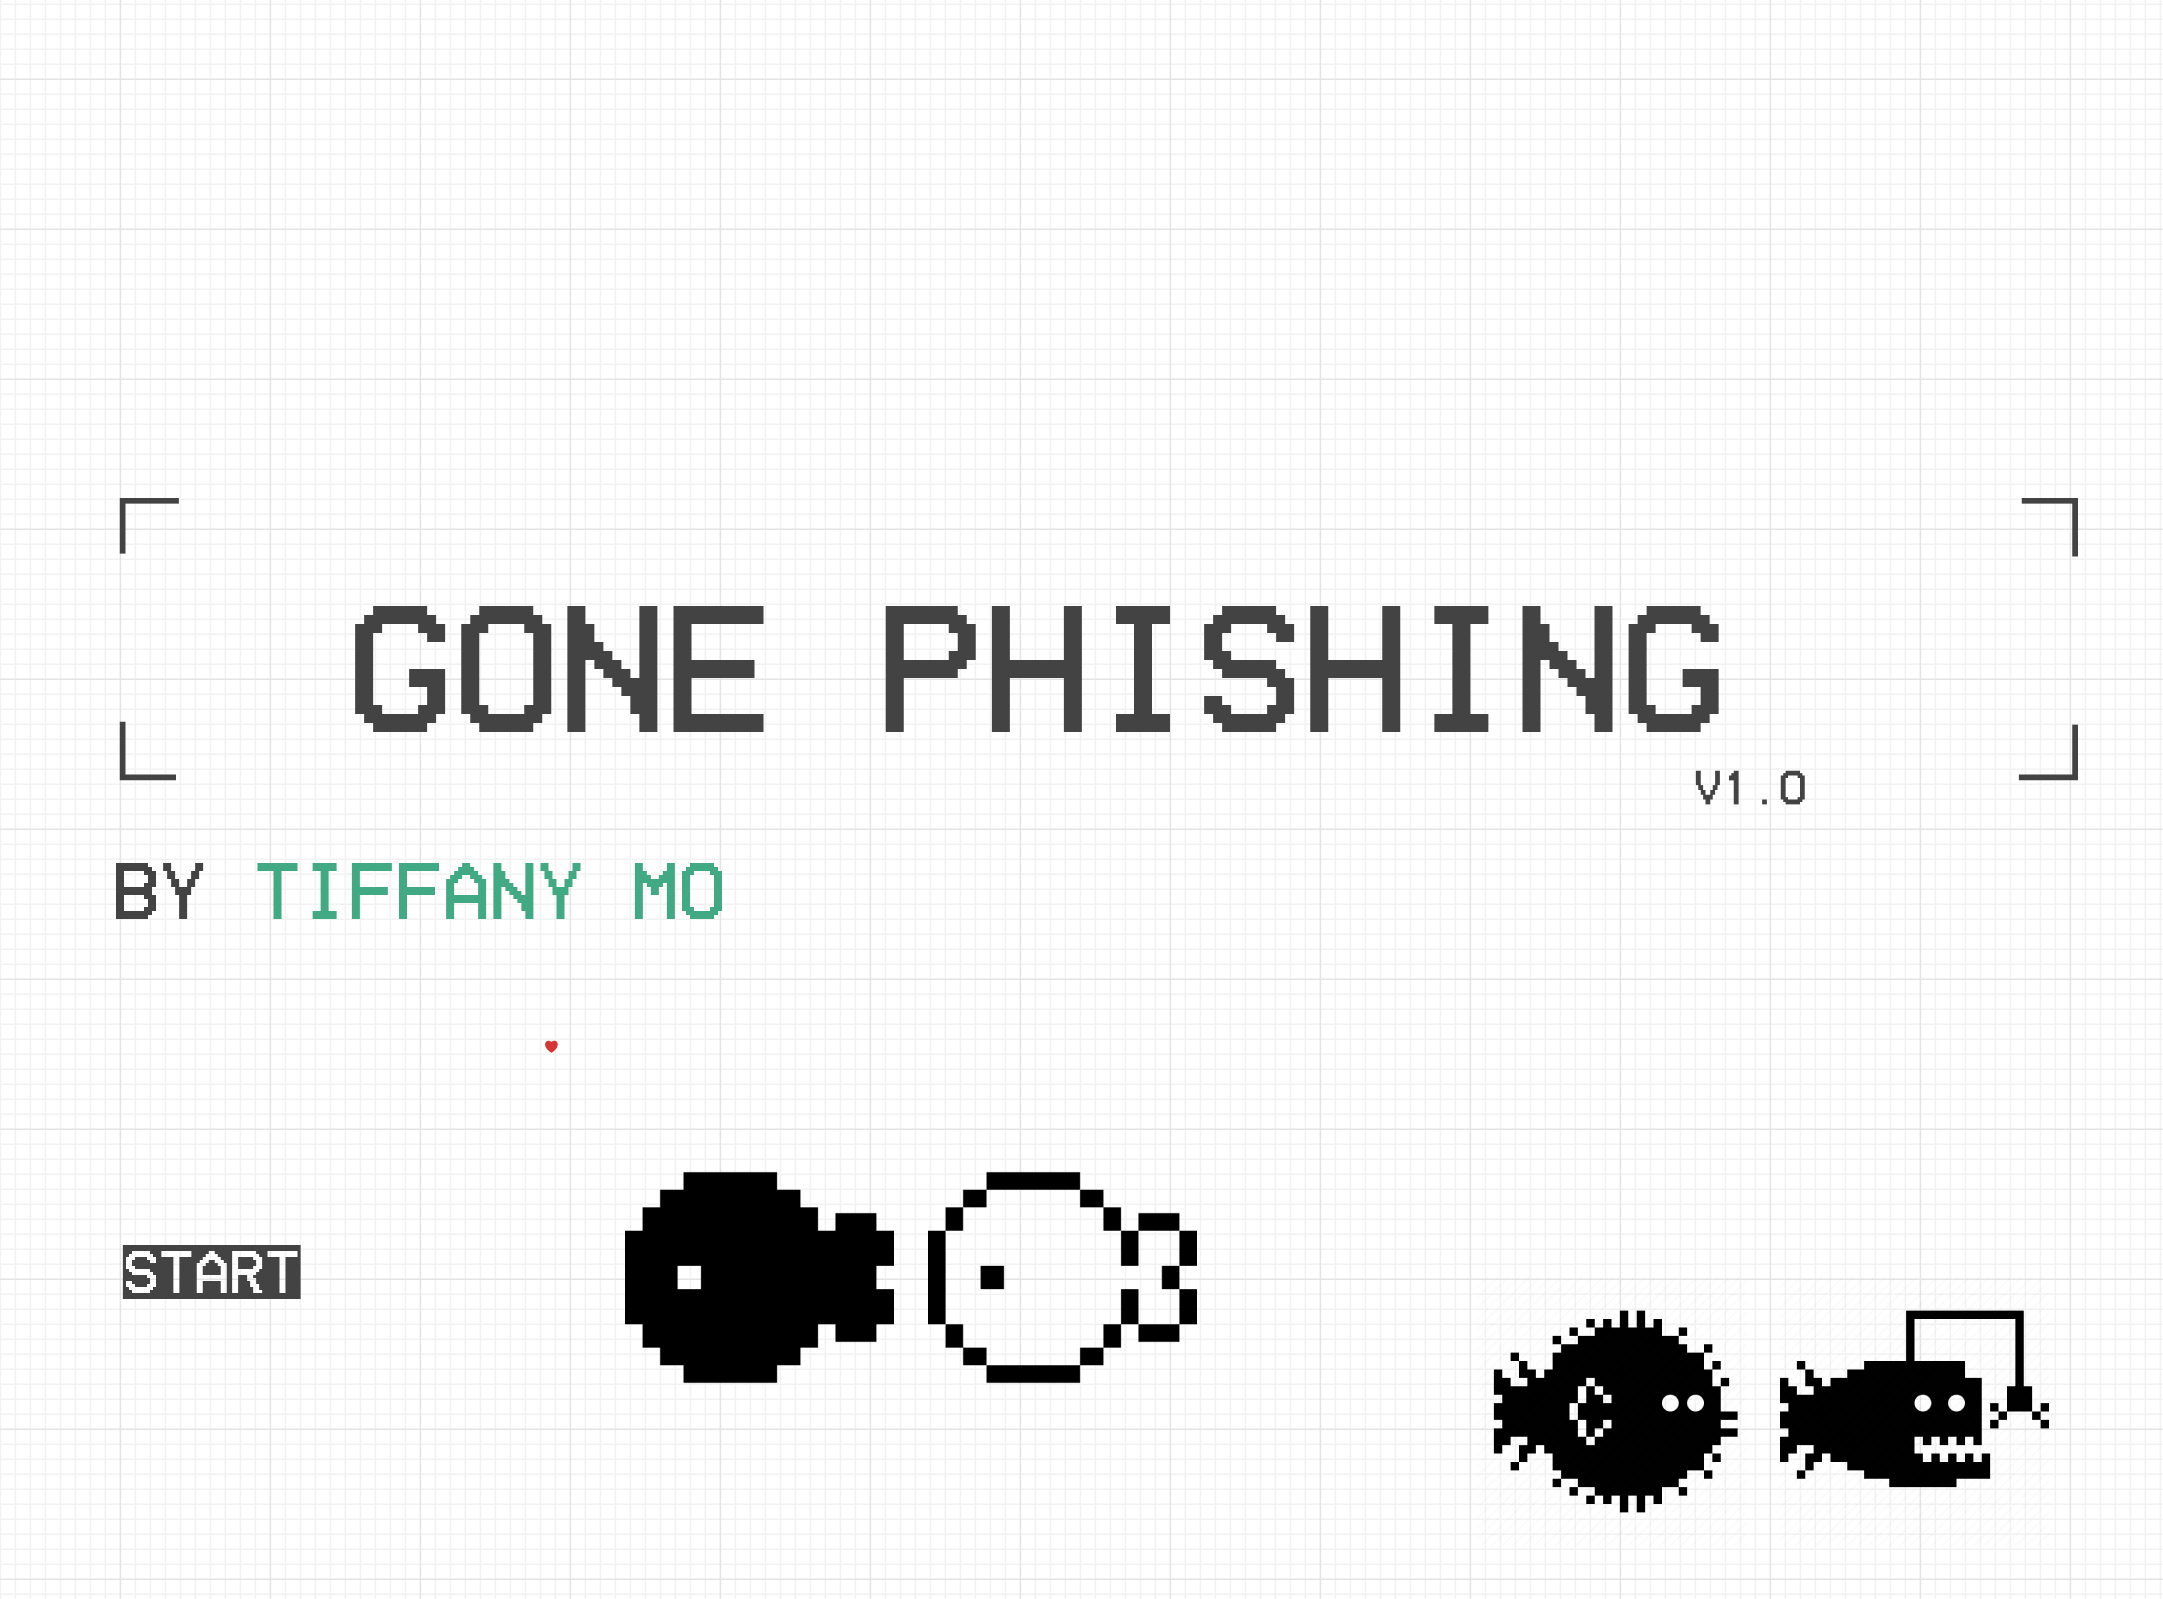
\includegraphics[scale=0.1]{PrototypeTitle.png}
\\
\textbf{Figure 1: Title Screen}
\\
\\ 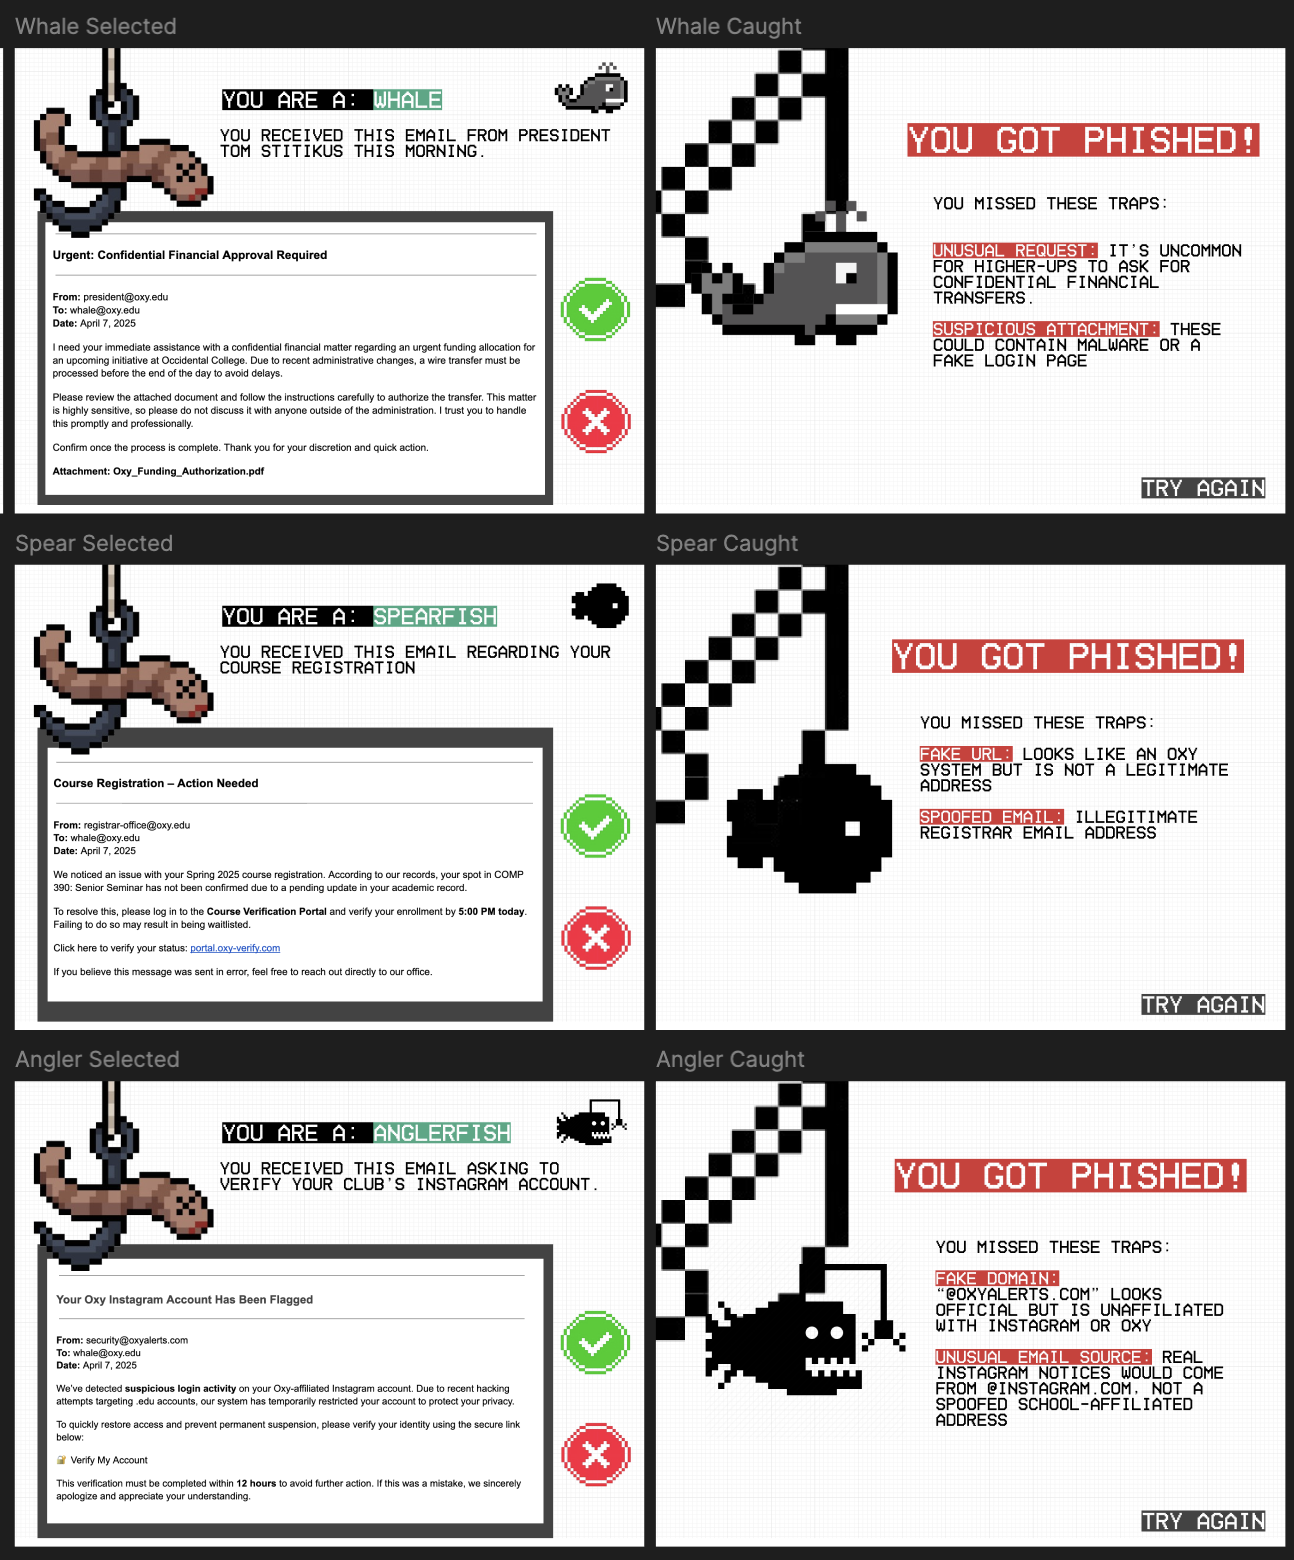
\includegraphics[scale=0.35]{prototypeFlow.png}
\\ \textbf{Figure 2: Email Approval and Lose Screen}
\\
\\While this prototype provides me some direction, several key components still need to be developed for the full version of my project. I will be prioritizing expanding the email dataset and developing a more detailed and story-like tutorial for a more comprehensive gameplay experience. I also plan to use this prototype to conduct initial user testing to assess my game’s educational effectiveness and identify areas for improvement.

\subsection{Evaluation Metrics}
To evaluate the success of Gone Phishing, I will focus on both functional performance and educational impact. On the functional side, my game should successfully generate contextually relevant phishing emails using GPT-4o based on real-world patterns drawn from the PhishTank dataset. The AI-generated content must load dynamically into the game, be displayed clearly to users, and trigger appropriate feedback and scoring logic based on player choices. Smooth integration between the React frontend, Node.js backend, and AI response handling will be a core technical metric. Additionally, the system should be secure (with no exposed API keys) and responsive, with no major usability bugs or performance issues.
From an educational perspective, I will evaluate success based on how well players understand and retain phishing awareness concepts after gameplay. To assess this, I will conduct user testing sessions with Oxy students, using a combination of observational testing, surveys, and post-game interviews. Each participant will first complete a brief pre-survey to gauge their baseline understanding of phishing and their confidence in identifying suspicious emails. They will then play a test version of Gone Phishing, where I will observe how they interact with the UI, whether they struggle to spot key red flags, and which types of phishing attacks they fall for most often.
Following gameplay, users will complete a post-survey measuring any changes in their phishing awareness, confidence levels, and understanding of specific tactics such as spear phishing, whaling, and angler phishing. I will also include a few reflection questions asking them to describe what made certain emails suspicious or believable. Optional follow-up interviews may be conducted for deeper feedback on the user experience and educational value. I will compare pre- and post-test responses to look for measurable improvements and use qualitative data to assess whether the game feels engaging, realistic, and instructive. This mixed-methods approach will help ensure that Gone Phishing is not just technically sound but also meaningfully improves phishing literacy among students.

\subsection{Timeline}
The following is my proposed timeline for next semester.
\begin{itemize}
  \item August:
    \begin{itemize}
        \item First week of class: Finalize project plan, clarify tech stack, set up development environment.
        \item Goal: Be technically ready to build and clear on project scope.
    \end{itemize}
    \item September:
    \begin{itemize}
        \item First milestone: Set up Node.js server and API route for GPT-4o email generation
        \item Second milestone: Set up basic React frontend
    \end{itemize}
    \item October:
    \begin{itemize}
        \item First milestone: Integrate GPT-4o prompts for 3-5 email types 
        \item Second milestone: Design core gameplay loop 
    \end{itemize}
    \item November:
    \begin{itemize}
        \item First milestone: Start conducting user testing 
        \item Second milestone: Polish UI, animations, and flow based on feedback
    \end{itemize}
    \item December:
    \begin{itemize}
        \item First milestone: Prepare and gather poster materials
        \item Second milestone: Collect feedback on realism, usability, and learning outcomes
        \item Third milestone: Finalize project, documentation, and completed comps report
    \end{itemize}
\end{itemize}

\section{Ethical Considerations}
\subsection{AI Phishing}
Research shows that \text{60\%} of participants fell victim to AI-automated phishing, comparable to human phishing messages created by experts. There are five phases of crafting a phishing scheme: identifying the target group, collecting data on the target, developing emails, sending emails, and validating and improving the emails. LLMs allow attackers to automate each of these steps with greater quality and quantity and less time and money. Phishing is an ideal task for LLMs because they both share a goal of creating realistic content from just a few data points about the target. 

\text{SNAP\_R} is an AI system that employed a clustering algorithm and a long short-term memory neural network to generated targeting phishing tweets. Despite only being able to produce basic tweets, the results showed that \text{SNAP\_R} could generate phishing tweets six times as fast as a human while maintaining a similar click rate(LLM effective). These results highlight the potential AI has to augment phishing campaigns. AI-powered phishing campaigns have already been observed in action. Darktrace observed a 135 increase in novel social engineering attacks among thousands of customers between January and February 2023 that were attributed to the rise of the widespread use of chatbots like ChatGPT.\cite{llm_vs_human}

\subsection{Environmental Impact}
Using Claude, a hacker could generate a batch of 1000 spear phishing emails for a cost of just \text{\$10 USD} in under 2 hours. However, one LLM query can require up to 10 times as much electric to process as a Google search. The increased demand of electricity will require data centers to expand by \text{60\%} by 2030. A study conducted by the University of Massachusetts Amherst concluded that training a single AI model can emit over 284,000 kilograms of carbon dioxide. This is equivalent to the amount of carbon dioxide produced by the entire lifetimes of 5 different cars. Training AI models not only emit carbon dioxide, but also require massive amounts of water to cool the machines used to train them. An approximate of 700,000 liters of water was used for cooling in the process of training ChatGPT-3 at Microsoft’s facilities. 
The usage of any AI system will have direct and indirect environmental effects. The production, transport, operations, and end-of-life stages of computer resources are energy-intensive and cause substantial greenhouse gas emissions and resource consumption. These are direct impacts. On the other hand, indirect impacts may result from AI usage in sectors like mining and manufacturing, where efficiency gains paradoxically increase greenhouse gas emissions. AI’s potential for efficiency and the loss of human labor comes at the expense of exacerbating environmental issues. As AI’s computational ablity expands, so will its energy demands. Research has predicted that a LLM assistant for Google searches could require an equivalent amount of energy as Ireland’s annual energy consumption. Its also important to note that the real emissions produced by major tech companies—Google, Microsoft, Meta, and Apple—were about \text{62\%} higher than officially reported from 2020-2022.\cite{ai_colonialism}

\subsection{LLM Regulation}
Currently, it is difficult for policymakers to mitigate misuse of LLMs due to the nature of AI training systems. The large, unsupervised volume of data used to train these models solicit unsupervised learning (LLM effective). Bceuase of this, it is difficult to limit LLM usage/capability to merely “positive” use, which can be subjective in itself. Thus, LLMs can be used by both parties, to both detect and and produce cyberattacks. As these AI models improve, new risks will emerge. For an LLM, the request tto produce phishing emails for a company phishing campaign may not be so different from one used for a marketing campaign. To reduce the likelihood of malicious users utilizing AI to cause harm or bypassing terms if service, LLMs can integrate structured access schemes, like application programming interfaces(APIs) to control the interactions between AI systems and users. One approach could include using a multiple layers of LLMs in order to recognize and catch risky user prompts. High risk queries, like those suspected to be used for legitimate phishing attacks, can then undergo a second round of validation by a more sophisticated model to analyze user input for malicious intent and flag users.\cite{llm_vs_human} 

\subsection{Accuracy}
A study found that phishing emails that were created using a combination of GPT and the V-triad had the highest success rate above fully AI-generated or human-generated phishing emails.\cite{llm_vs_human} They concluded that semi-automation is significantly useful and a viable option for creating phishing campaigns while remaining accurate. This significantly lowers the time and knowledge needed, while providing results as good, or even better, than manually created emails. Using a one-size-fits-all approach is ineffective for helping users prevent being phished. What makes one person avoid phishing emails makes another person fall for them. These tactics need to be personalized. LLMs help to achieve personalization and tailored user content using just a few data points while avoiding human error. 
However, even if computers can avoid human errors, they aren't exempt to their own errors. It has been well-known that generative AI tend to "make things up." This is what makes generative AI such a novel tool. No matter what the prompt, AI has the inventive capacity to sound totally confident and make statements that often agree with the user's claims. This is because LLMs tend to blur truth and fiction, inserting incorrect details into seemingly factual sentences. Computer scientists refer to these sentence-filling mistakes as "hallucinations." 
Fundamentally, LLMs were not designed to simply generate facts. They compose responses that are statistically likely based on patterns in their training data. Despite fine-tuning and rigorous testing, it is impossible to make out the true internal workings of an LLM and how they produce their responses. When AI models are trained, they squeeze the relationships between tens of trillions of words into billions of parameters. Co founder of Vectara, a Palo Alto company, says “Amazingly, they’re still able to reconstruct almost \text{98\%} of what they have been trained on, but then in that remaining \text{2\%}, they might go completely off the bat and give you a completely bad answer”. 
To reduce AI hallucinations, developers use several strategies. Larger and longer-trained models hallucinate less but are costly and may sacrifice other abilities. Cleaner, larger datasets help but are limited in availability. One key method is retrieval-augmented generation (RAG), where chatbots refer to trusted sources, improving factual accuracy in areas like medicine and law—though RAG isn’t flawless, as it can't cover all possible knowledge. Another method involves using separate systems to fact-check AI responses via internet searches, like Google Gemini’s double-check tool, which verifies content with color coding. However, this is slow, expensive, and still vulnerable to unreliable online data.\cite{hallucinate}

\section{Results and Discussion}
In this section, I plan to consolidate my findings from the evaluation metrics in order to draw conclusions on the effectiveness of this project. 







\appendix



\printbibliography 



\end{document}
